\title{Star Formation, Feedback, and Chemical Evolution of Dwarf Galaxies}

\author{PI: Mordecai-Mark Mac Low, American Museum of Natural History, New York.\\
        co-PI: Andrew Emerick, Columbia University / AMNH }

\documentclass[11pt]{article}

\usepackage[letterpaper, margin=1in]{geometry}
\usepackage{amsmath}

\usepackage{natbib}
\usepackage{multirow}
\usepackage{multicol}
\usepackage{array}
\usepackage{graphicx}
\usepackage{epstopdf}
%\usepackage{siunitx}
\epstopdfsetup{update}
\newcolumntype{L}{>{\centering\arraybackslash}m{2cm}}
\newcolumntype{R}{>{\centering\arraybackslash}m{1.25cm}}

\renewcommand{\floatpagefraction}{.8}%

\citestyle{aa}

\newcommand {\apj}{ApJ}
\newcommand {\aj}{AJ}
\newcommand {\apjs}{ApJS}
\newcommand {\apjl}{ApJL}
\newcommand {\mnras}{MNRAS}
\newcommand {\aap}{A\&A}
\newcommand {\aapr}{A\&ARv}
\newcommand {\araa}{ARA\&A}
\newcommand {\pasj}{PASJ}
\newcommand {\pasp}{PASP}
\newcommand {\bain}{Bulletin of the Astronomical Institutes of the Netherlands}
\newcommand {\fcp}{Fundamentals of Cosmic Physics}
\newcommand {\nat}{Nature}
\newcommand {\na}{New Astronomy}
\newcommand{\eg}{e.g.,}
\newcommand\rmxaa{Rev. Mex. Astron. Astrofis.} % Revista Mexicana de Astronomia y Astrofisica

%\DeclareSIUnit\parsec{pc}
\newcommand{\msun}{$\textrm{M}_{\odot}$}
\newcommand{\rsun}{$\textrm{R}_{\odot}$}
\newcommand{\lsun}{$\textrm{L}_{\odot}$}

\begin{document}
\maketitle

\section{Introduction}
This renewal proposal describes our proposed research for the coming year. We focus on using a new, detailed model for stellar feedback physics to understand the dynamical and chemical evolution of low mass dwarf galaxies. This project is a novel endeavor in galaxy-scale simulations as our method uses particles to trace individual stars in our galaxy, rather than averaging whole stellar populations into a single particle. This allows us to follow the feedback physics of individual stars in unprecedented detail -- including realistic models for stellar winds, supernovae, diffusive stellar heating, and radiative transfer -- with parsec scale resolution. In addition, we use this new formalism to follow ejected elemental yields from individual stars, allowing us to trace stochastic variations in local and galactic scale chemical abundances for over a dozen different elements. The PI of this proposal (M-M. Mac Low) is PI on NSF grant AST11-09395 and co-PI Emerick is supported by a NSF Graduate Research Fellowship (DGE-16-44869); this project is co-advised by collaborator G. Bryan. We summarize the science motivation for each of these projects below, while justifying our resource request. We note that this project is central to the Ph.D thesis of co-PI Emerick.

\subsection{Star Formation, Feedback, and Chemodynamics of Galaxies}

Recently, large scale, cosmological hydrodynamics simulations have been able to reproduce many observed, integral properties of galaxies over a wide range of galaxy stellar masses and dark matter halo masses \citep[\eg][]{MUGS2010, MAGICC2013, Illustris1, Illustris2, OWLS, EAGLE, FIRE, APOSTLE, Latte}. 
%mm [redundant with following sentence]  These works have made strides in reconciling outstanding disagreements between predictions from $\Lambda$CDM cosmology and observations of nearby dwarf galaxies. 
Improvements in our understanding of baryonic physics, most importantly understanding the importance of stellar feedback in the self-regulation of star formation in galaxies, has allowed these works to reconcile many outstanding disagreements between predictions from $\Lambda$CDM cosmology and observations of nearby dwarf galaxies. However, due to computational constraints, feedback implementations are usually phenomenological, tuned to reproduce observed galaxy properties. Clearly, given its role in galaxy evolution, a deeper understanding of feedback physics is needed. This can be gained through high resolution, idealized simulations of individual galaxies. We propose to conduct a sensitive test of how various feedback processes affect galaxy evolution in order to self-consistently reproduce dynamical, morphological, and chemical properties of dwarf galaxies simultaneously. We will conduct high resolution simulations of a set of small dwarf galaxies, varying the underlying feedback physics, while, for the first time in a galaxy scale simulation including well-resolved feedback, tracing chemical abundances and stellar evolution on a star-by-star basis.

Historically, inclusion of feedback physics in galactic scale simulations meant the injection of purely thermal energy in a localized region---often with tricks to prevent rapid, unphysical overcooling of gas---to model the effects of supernovae explosions. It has become clear that feedback physics must be implemented in much greater detail than this, simultaneously considering multiple, distinct types of feedback energy. In addition to energy injection from core collapse and Type Ia supernovae, we will include the effects of 1) energy injection from the winds of both massive and AGB stars, 2) radiation feedback (photoionization, photoheating, and radiation pressure) from massive stars followed directly using adaptive ray tracing, 3) a model for photoelectric heating of dust grains due to stellar radiation, and 4) stellar Lyman-Werner (LW) radiation that can destroy regions of molecular hydrogen. The effect of these feedback sources on the chemical evolution of galaxies will provide a new dimension of analysis and observational comparisons not often considered in these types of simulations.

In general we have a fair understanding of the mean chemical properties of galaxies, but models have difficulty in reproducing the observed scatter in both gas phase and stellar abundances. In particular, models of the chemical evolution of dwarf galaxies are often tuned to match the observed properties of a small number of observed galaxies. Self-consistently reproducing both the dynamic and chemical, or chemodynamical, properties of dwarf galaxies in hydrodynamics simulations remains a standing challenge for theoretical models. In addition, with one exception \citep{Few2012, Few2014}, all hydrodynamics simulations examining galactic chemodynamics to date have been implemented in smooth particle hydrodynamics (SPH) codes. Although historical problems with the SPH formalism have been ameliorated substantially in recent years, they often still employ sub-grid mixing schemes to model mixing of spatially adjacent but chemically inhomogeneous gas \citep[\eg][]{ShenWadsleyStinson2010}. In part due to these methods, there are outstanding uncertainties in how much results depend on specific code implementations \citep{Revaz2016}. In addition, using star particles that represent clusters of stars becomes problematic at the high spatial and particle mass resolution needed for simulating low mass dwarf galaxies \citep{Revaz2016}. 

This motivates our development and use of a new method for studying galactic chemical evolution in hydrodynamics simulations, including, for the first time, a broad range of feedback physics, while also following individual stars down to the solar mass range. This is particularly exciting with recent or ongoing---for example ANGST \citep{ANGST2009}, APOGEE \citep{APOGEE2010}, and GAIA---and upcoming observational studies (e.g. APOGEE-2) that will obtain stellar abundance measurements in both the Galaxy and nearby dwarfs. These will provide ideal comparisons to our simulations of dwarf galaxies with individual, chemically tagged stars.

We provide a discussion of the feedback physics and associated models we propose to include in our simulations. We seek to understand how each of these processes individually and together affect galactic dynamical and chemical structure. 

%\section{(better name needed) Technical Goals}

\section{Galaxy Star Formation and Feedback Physics}

In this section we outline the multitude of base physical processes in our simulations that serve to capture a realistic galaxy scale ISM and star formation conditions. In addition, we outline the individual components and justifications for each portion of our included feedback physics.

The following constitutes the core set of physical processes used in our simulations that will be held fixed in each simulation: 1) gas self-gravity to capture gas collapse and subsequent star formation in dense regions, 2) a nine-species, non-equilibrium chemistry solver, following electrons, and H, He, and H$_{2}$ and their ionization states \citep{Anninos1997, Abel1997}, 3) associated heating / cooling as followed in the \texttt{Grackle} library \citep{Grackle}, including heating from a metagalactic UV background \citep{HM2012} and tabulated metal line cooling from \texttt{Cloudy} \citep{Cloudy2013}, 4) approximate H and He gas self-shielding of the UV background \citep{Rahmati2013}, 5) a metagalactic Lyman-Werner (LW) flux from \cite{HM2012} to properly model H$_{2}$ dissociation with approximate H$_{2}$ self-shielding \citep{Wolcott-Green2011}, and 6) a collisionless N-body solver to evolve the dynamics of the formed star particles. In every simulation, we form stars from dense gas on the most refined parts of the grid (with resolution of 1.5~pc) following a stochastic star formation scheme from \cite{Goldbaum2015, Goldbaum2016}, modified to sample individual stellar masses from an input IMF \citep[e.g.][]{Salpeter1955}. We use a high star gas density threshold for star formation, $n > 10^{3}$ cm$^{-3}$, and do not force a pre-defined star formation efficiency per free fall time in order to test whether or not these feedback processes are capable of self-regulating star formation to the expected efficiency of $\sim$ 2\% \citep{Kennicutt1998}; this is similar to what has been done successfully in the FIRE feedback simulations \citep[e.g][]{FIRE}. Each star is chemically tagged by the local gas abundances, and assigned stellar properties from a grid of stellar evolution tracks \citep{Bressan2012}, which ultimately govern the stellar radiative properties, wind velocity, and the star's lifetime. We follow the mass loss of each particle via stellar winds and supernovae over time as determined by our stellar yield model.

Supernovae and stellar wind feedback -- the sources of ejected stellar yields -- will be treated uniformly in each simulation. Stellar yields for both winds and supernovae are taken from the NuGrid data set \citep[][Ritter et. al. in prep]{Pignatari2016}, a self-consistent model of stellar yields over a well sampled range of stellar masses ($M_{*} \in [1,25]~M_{\odot}$) and metallicities ($Z\in [10^{-4},0.02]$). We model stellar winds from massive stars ($M > 8~M_{\odot}$) using a constant mass loss rate over their lifetime, while low mass stars ($M < 8~M_{\odot}$) remain quiescent until a final AGB phase wind emitted near the end of their lives. Stellar properties, including lifetimes,  start of a star's AGB phase, radius, surface gravity, and effective temperature are obtained via interpolation over the \texttt{PARSEC} grid of stellar evolution tracks \citep{Bressan2012}\footnote{Stellar radius, surface, gravity, and effective temperature are used only for determining radiation properties of our stars, and play no direct role in our simulations}. Massive stars (M $>$ 8 M$_{\odot}$) explode as core collapse supernovae at the end of their lives; however, the final fate of stars above 25 M$_{\odot}$ is uncertain, and likely varies non-trivially with stellar metallicity. We track stellar winds from these stars using the yields from Slemer et. al. (in prep), and adopt the simple assumption that these stars form a direct collapse compact object at the end of their lives, with no mass ejection. Stars below 8 M$_{\odot}$ are tracked after their death as white dwarf particles, assigning white dwarf masses from the observed initial-to-final-mass distribution \citep{Salaris2009}. Following \citep{Cote2015}, we use an observationally motivated delay time distribution model \citep[\eg][]{Maoz2014} to assign to each white dwarf a time when they will explode as a Type Ia supernova.\footnote{We note that only a few percent of white dwarfs should explode as Type Ia in a Hubble time \citep{Maoz2014}; our model takes this into account in assigning explosion times, with a large majority never exploding.} We adopt Type Ia supernova yields from \cite{Thielemann1986}.

%Accounting for the effects of CRs in galaxy scale simulations has only been possible recently, yet is likely a very important source of additional feedback in galaxies \citep[\eg][]{SalemBryan2014, SalemBryanHummels, SalemBryanCorlies, GirichidisCR, Pakmor2016, Simpson2016}. The role of CRs in low mass dwarf galaxies is still uncertain, though has been investigated recently in more massive dwarfs than those considered in this proposal \citep{Chen2016}. The implementation of CR feedback in \texttt{Enzo} \citep{SalemBryan2014} assumes both isotropic diffusion and ignores energy losses from interactions with an ordered magnetic field. Isotropic diffusion in very low mass dwarf galaxies may not be a poor assumption, as their lack of obvious disk structure may indicate that they lack the ability to create a global, ordered magnetic field that would cause anisotropies in CR behavior. We inject CR energy during supernova explosions at 10\% of the total energy injected, reducing the subsequent thermal / kinetic energy injection accordingly. CRs in our simulations diffuse isotropically as controlled by a diffusion coefficient, and interacting with the hydrodynamics through an additional, non-thermal pressure term.

Radiation from massive stars provides a substantial additional source of feedback in galaxies \citep[\eg][]{Agertz2013}. Including radiative feedback has a significant affect on galaxy dynamical and morphological structure \citep[\eg][]{WiseAbel2012, Kim2013a, Kim2013b, Roskar2014, Rosdahl2015}. Radiation fluxes for each of our stars are computed using the \texttt{OSTAR2002} grid of stellar atmosphere models \citep{Lanz2003}; for stars with effective temperatures below those sampled on the \texttt{OSTAR2002} grid, we compute radiation rates assuming a black body spectrum, scaled to be consistent with the \texttt{OSTAR2002} models. In this proposal, we include radiative feedback in three distinct forms: 1) H and He ionizing radiation from massive stars, 2) local FUV flux from massive stars that contribute to photoelectric heating within the ISM, and 3) local LW flux from massive stars that regulate H$_{2}$ formation and dissociation. 
%Separating these physics will allow us to directly address recent disagreement in the role of photoelectric heating in dwarf galaxies \citep{Hu2016, Forbes2016}. 
We use \texttt{Enzo}'s radiative transfer capabilities \citep{Wise2012a,WiseAbel2012,Wise2014} to track ionizing radiation directly, coupling the ionizing / heating rates to the \texttt{Grackle} chemistry solver, and accounting directly for the effects of Hydrogen radiation pressure. We assume the FUV radiation to be everywhere optically thin and apply a photoelectric heating rate model from \cite{BakesTielens1994} and \cite{Wolfire2003} that scales with local density, temperature, and metallicity. Finally, we track stellar LW radiation in the optically thin limit, but include an approximate H$_{2}$ self-shielding prescription.

\section{Computational Method and Model Descriptions}

Our dwarf galaxy simulations will be carried out using \texttt{Enzo}\footnote{www.enzo-project.org}, an adaptive mesh refinement (AMR) hydrodynamics and N-body code. \texttt{Enzo} is an entirely open-source code that is undergoing active development by many researchers across several institutions; its most recent stable release is version 2.5. This project involves a substantial amount of additional code development built on top of the development version of \texttt{Enzo} (version 2.X)\footnote{This version is also publicly available at www.bitbucket.org/aemerick/enzo-emerick}. \texttt{Enzo} has been well tested and extensively used in a variety of applications, including the ISM \citep{2005MNRAS.356..737S, 2008ApJ...673..810T}, the IGM \citep{2000ApJ...534...57B, 2001ApJ...561L..31F}, the first stars and galaxies \citep[\eg][]{Wise2012a, WiseAbel2012, Wise2014}, and the roles of various feedback methods in galaxies \citep[\eg][]{Simpson2015, SalemBryan2014, Goldbaum2016, Forbes2016}. We outline the methods employed in \texttt{Enzo} as relevant to our proposal; a detailed description of these methods can be found in the \texttt{Enzo} method paper \citep{Enzo2014}. 

We will conduct a controlled set of numerical experiments on the effect of various feedback physics on a set of three dwarf galaxies with varying initial gas masses, each embedded in the same fixed dark matter potential. In each case, we initialize the dwarf galaxy as a spheroidal distribution of gas in hydrostatic equilibrium with a dark matter halo of virial mass 10$^{9}$ M$_{\odot}$, corresponding to a maximum circular velocity of about 10 km s$^{-1}$. Our smallest dwarf galaxy will have a total gas mass of $\sim 2 \times 10^{6}$ M$_{\odot}$, comparable to the total baryonic (stars and gas) mass of the Local Group ultrafaint dwarf galaxy Leo P \citep{McQuinn2013, Giovanelli2013, Skillman2013, McQuinn2015}. The gas phase abundances and metal retention in Leo P will form the basis of our direct comparison to observation \citep{McQuinn2015}. In addition, we will simulate two more massive galaxies with gas masses of $\sim 5 \times 10^{6}$ M$_{\odot}$ and $10^{7}$ M$_{\odot}$. Given that dwarf galaxies are effective at driving out a substantial amount of gas through stellar feedback \citep[e.g.][]{MacLowFerrara1999}, these more massive models are likely more representative of the total amount of gas Leo P has processed to form its observed $5.6\times 10^{5}$ M$_{\odot}$ of stars, corresponding to reasonable mass loading factors on order of 10 - 20. We will follow each of these gas clouds as they collapse, stopping each simulation 200 Myr after star formation. For each galaxy, we will run one simulation with full feedback physics (stellar winds, supernovae, and radiation), as well as one simulation without any radiation, for a total of six simulations at our fiducial resolution.

We center each dwarf galaxy on a uniform $128^3$ cell mesh with physical dimensions of $12.288^3$ kpc, corresponding to a root grid resolution of 96 pc. Additional levels of refinement are applied to regions surpassing a chosen density contrast, in addition to requiring the Jeans length be resolved to at least 16 cells. Each additional level of refinement increases the resolution by a factor of 2, allowing us to achieve 1.5 pc resolution with a total of 6 levels of refinement. In addition, we force refinement around all star particles, so that feedback injection is always resolved at the maximum refinement level. Ideally we would like to use higher resolution in order to completely resolve key aspects of the feedback physics (particularly relating to bubble formation from stellar winds and ionizing radiation); however this becomes exceedingly expensive to run for long timescales. With 200 Myr of evolution, we will be able to trace the evolution of gas phase abundances through the various phases of our dwarf galaxy's ISM, how effectively feedback ejects metals from the dwarf galaxy's disk, and whether or not realistic feedback is capable of unbinding this enriched gas from the dark matter halo.

%Such long timescales are essential to capture a long period of star formation evolution and chemical enrichment; $\sim$ 1 Gyr represents a few dynamical times in our dwarf galaxy, the time required to understand metal mixing across the galaxy. In addition, 1 Gyr is approximately the timescale over which the knee in the $\left[ \alpha / \rm{Fe}\right]$ vs. $\left[\rm{Fe}/\rm{H}\right]$ diagram appears, marking the time when substantial iron peak elemental enrichment from Type Ia supernovae begins. Capturing this knee is an important observational diagnostic.

Based on our tests at 1, 1.5, and 2 pc resolution, 1.5~pc resolution both adequately resolves these feedback physics, and remains computationally tractable to run for our required timescales. \texttt{Enzo} helps reduce overall expense by using adaptive time steps, evolving each refinement level independently with the timestep size set by the Courant-Friedrichs-Levy condition for numerical stability for that level. The exact size of each step is thus dependent on the sound speed and gas velocity in zones at that level. Since supernova can heat the ISM to temperatures on order of 10$^{6-7}$ K, and stellar winds have velocities on order of 10$^{3}$ km s$^{-1}$, we expect typical timesteps of about 600 years on our most refined level. A majority of the time spent computing a given cycle will be spent on the most refined level, as our tests show we should expect root grid time steps on order of 0.25 Myr.

We couple \texttt{ENZO} to the open-source \texttt{Grackle} chemistry and heating/cooling library, which operates cell-by-cell on each grid. \texttt{Grackle} sub-cycles through a non-equillibrium chemistry solver following methods first used in \cite{Anninos1997} and \cite{Abel1997} that solve for the correct densities and ionization states of each species, while accounting for radiative cooling and heating from external radiation fields. This allows us to self-consistently couple our 9 species chemistry network with the heating/cooling effects from the metagalactic background, and galactic ionizing, far-ultraviolet, and LW radiation fields.
%mm , and  photoelectric heating from the far-ultraviolet radiation field.

%CR's are traced using the two-fluid approximation implemented in \cite{SalemBryan2014}. The CRs are treated as a secondary fluid coupled to the hydrodynamics through a pressure term, acting as an additional, non-thermal pressure source. CR diffusion is computed with an explicit finite difference scheme, which places an additional constraint on the size of each timestep, though the impact of this constraint is reduced somewhat by subcycling over the CR evolution. The CR timestep scales with the square of the cell size and is inversely proportional to the adopted diffusion coefficient. For a diffusion coefficient of $3\times10^{28}$~cm$^{2}$~s$^{-1}$, this corresponds to a reduction of a factor of $\sim$5 in our typical time step size over runs without CR's. For example, we expect typical time steps of $\sim$600 yr due to stellar winds at 1.5 pc resolution; including CR's, the diffusion limited timestep at this resolution is 112.5 yr at maximum resolution. We note that this impact is greatest at the highest refinement level: the hydrodynamics timestep decreases by a factor of two with doubled resolution, while the CR diffusion substep decreases by a factor of four, showing the need for subcycling.

We use the direct ray tracing algorithm described by \cite{WiseAbel2011} in \texttt{Enzo} to directly follow the H~{\sc i} and He~{\sc i} ionizing radiation from massive stars. This is an adaptive ray tracing method that splits rays using mapping on a \texttt{HEALPix} grid. These methods are well tested and have been used previously in cosmological simulations of reionization in the early Universe \citep{Wise2012a, WiseAbel2012,Wise2014, Kim2013a, Kim2013b}. These methods have been demonstrated to scale to $\mathcal{O}(10^{3})$~processors for large domains (up to $\sim 10^9$ cells) and many sources ($\sim10^{4}$). Although we expect $\sim$100-500 sources at any one time in our simulations, direct ray tracing does still incur a significant additional expense. We mitigate this additional expense by allowing rays to merge once they are far from their source, and using a reduced speed of light approximation (though we are capable of running without this simplification); neither of these approximations should significantly affect results in an isolated galaxy simulation. 
%As discussed in our supplemental code scaling document, with these approximations we anticipate a slow down of a factor of 5--10 for our typical source count.

Figure~\ref{fig:dwarf galaxy} shows the results from two low resolution (8 pc) proof-of-concept simulations of our most massive dwarf galaxy model about 200 Myr after the onset of star formation. Shown are edge-on weighted projections of number density and integrated projections of O column density for a simulation run with full feedback physics (left column) as compared to one run without any stellar radiation feedback. Individual stars are marked with black dots in each image. There is substantial difference in these two simulations, already suggesting that radiation feedback is vital to properly simulation galaxy evolution, as there is an order of magnitude difference in stellar mass between these two galaxies. This dramatically influences the amount of metals produced in each galaxy (with the non-radiation simulation having much more), and it is obvious from these images that the full feedback physics simulation much more effectively removes gas and metals from this galaxy. Each of these simulations were run on 64 processors on the TACC Stampede cluster, where we propose to work. 

\begin{figure}
\centering
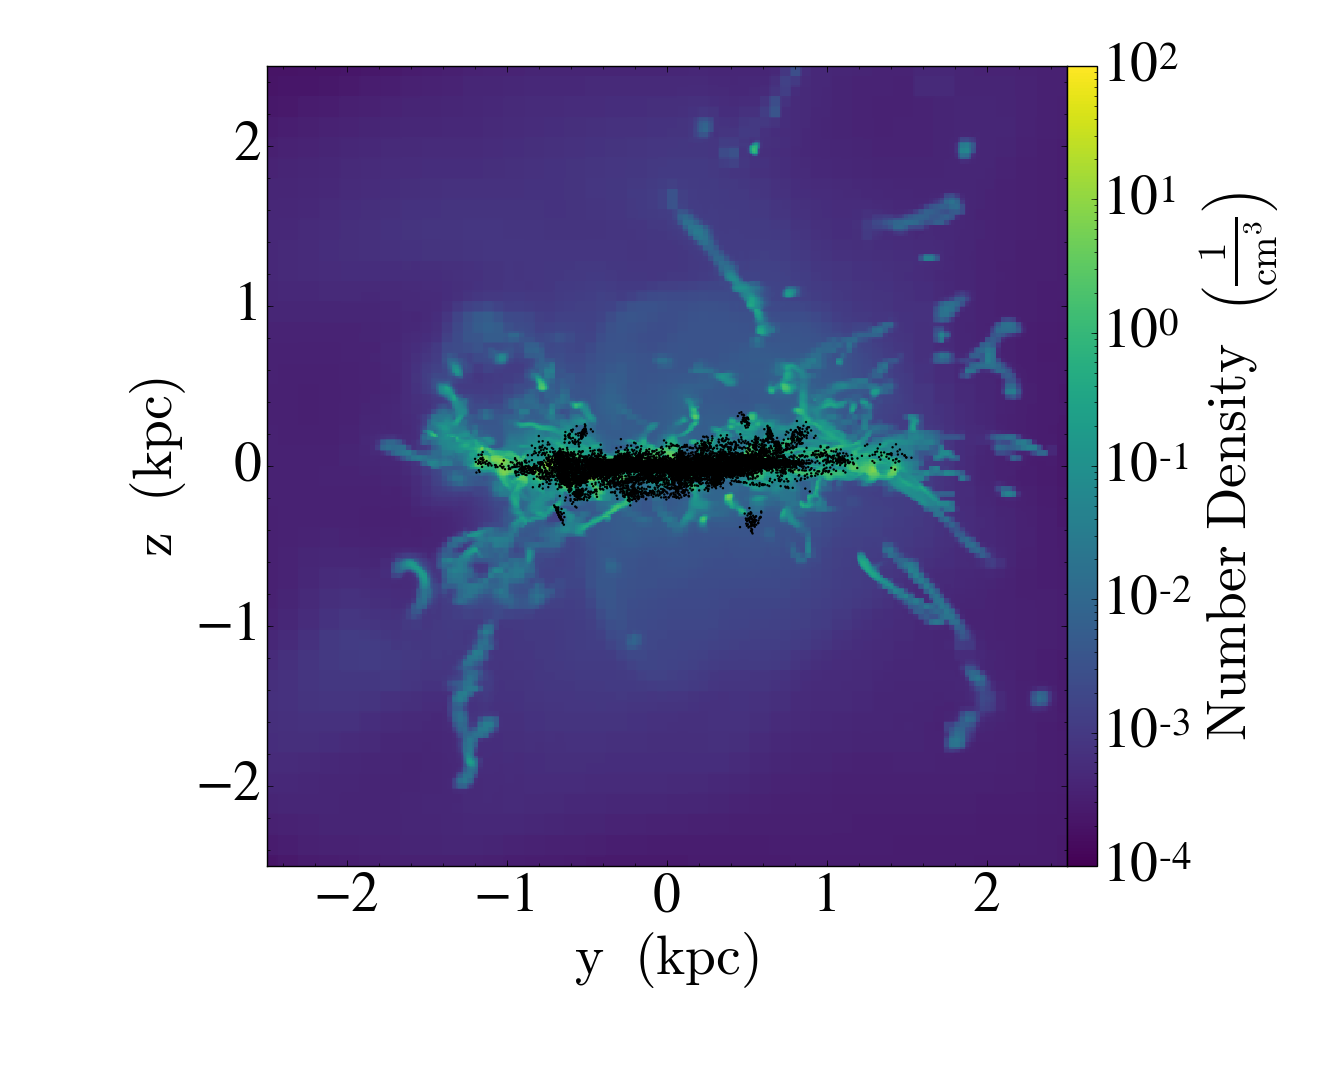
\includegraphics[width=0.4\linewidth]{number_density_proj_rad}
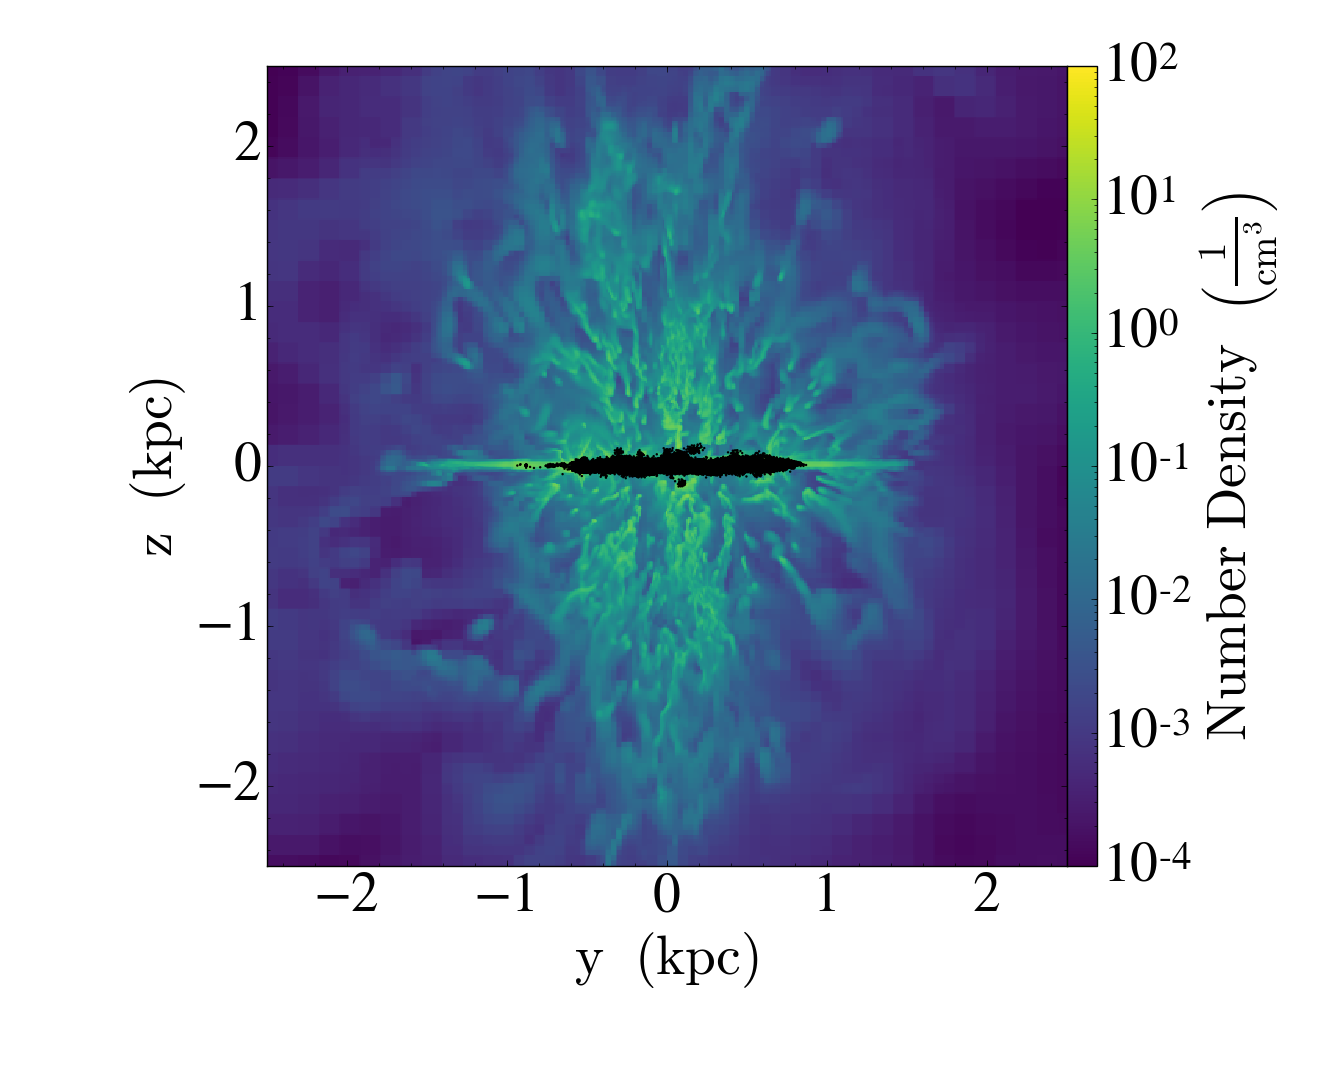
\includegraphics[width=0.4\linewidth]{number_density_proj_snwind}
\vspace{0.1cm}
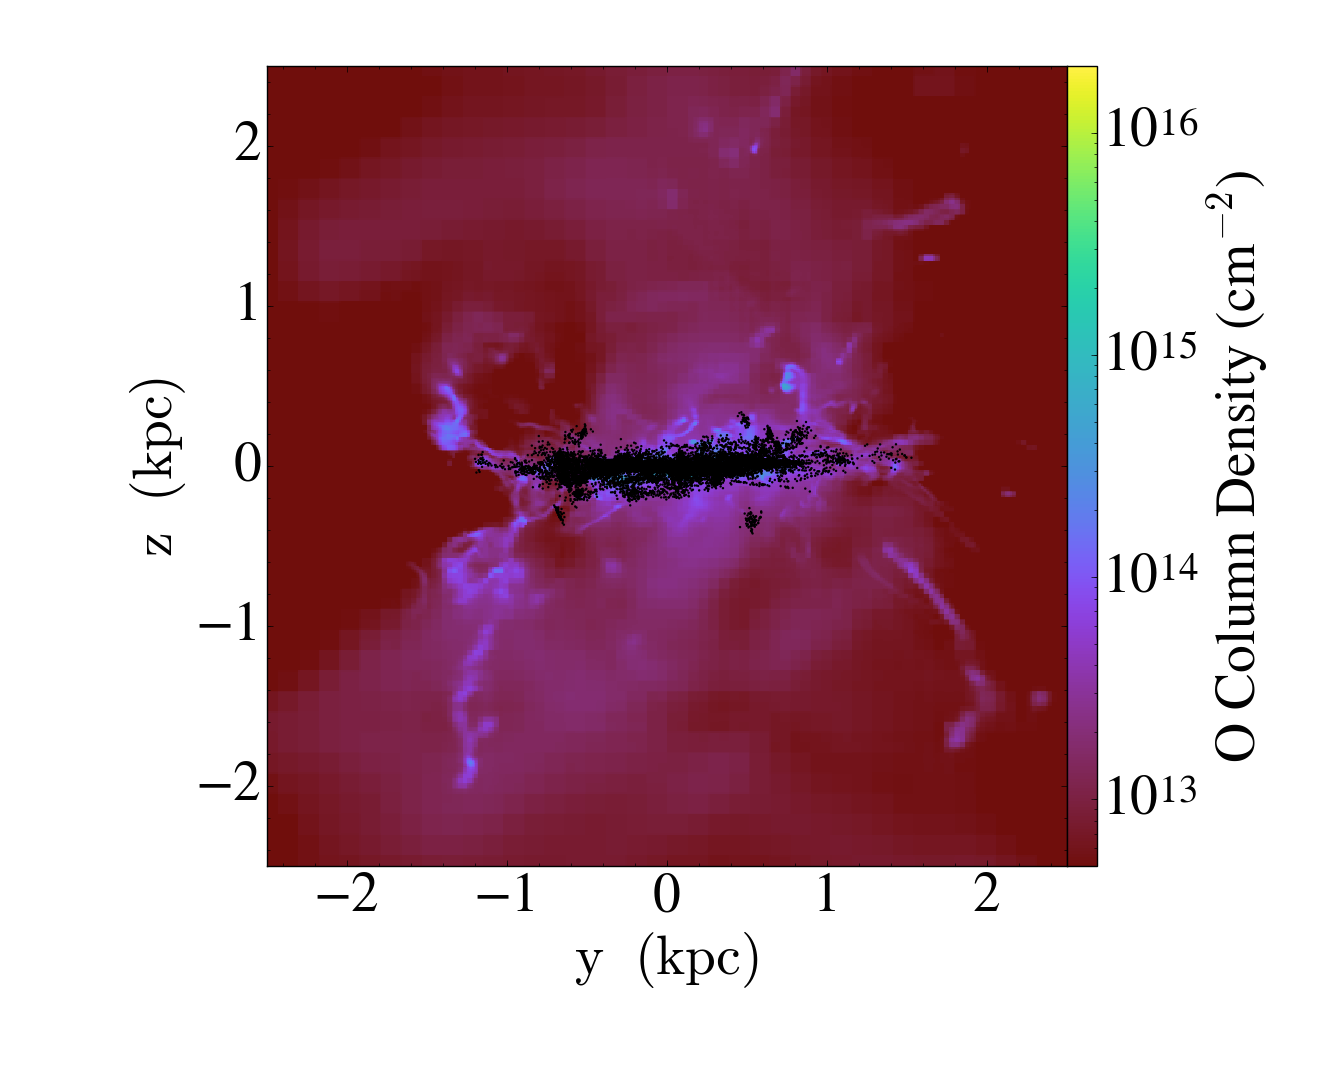
\includegraphics[width=0.4\linewidth]{O_proj_rad}
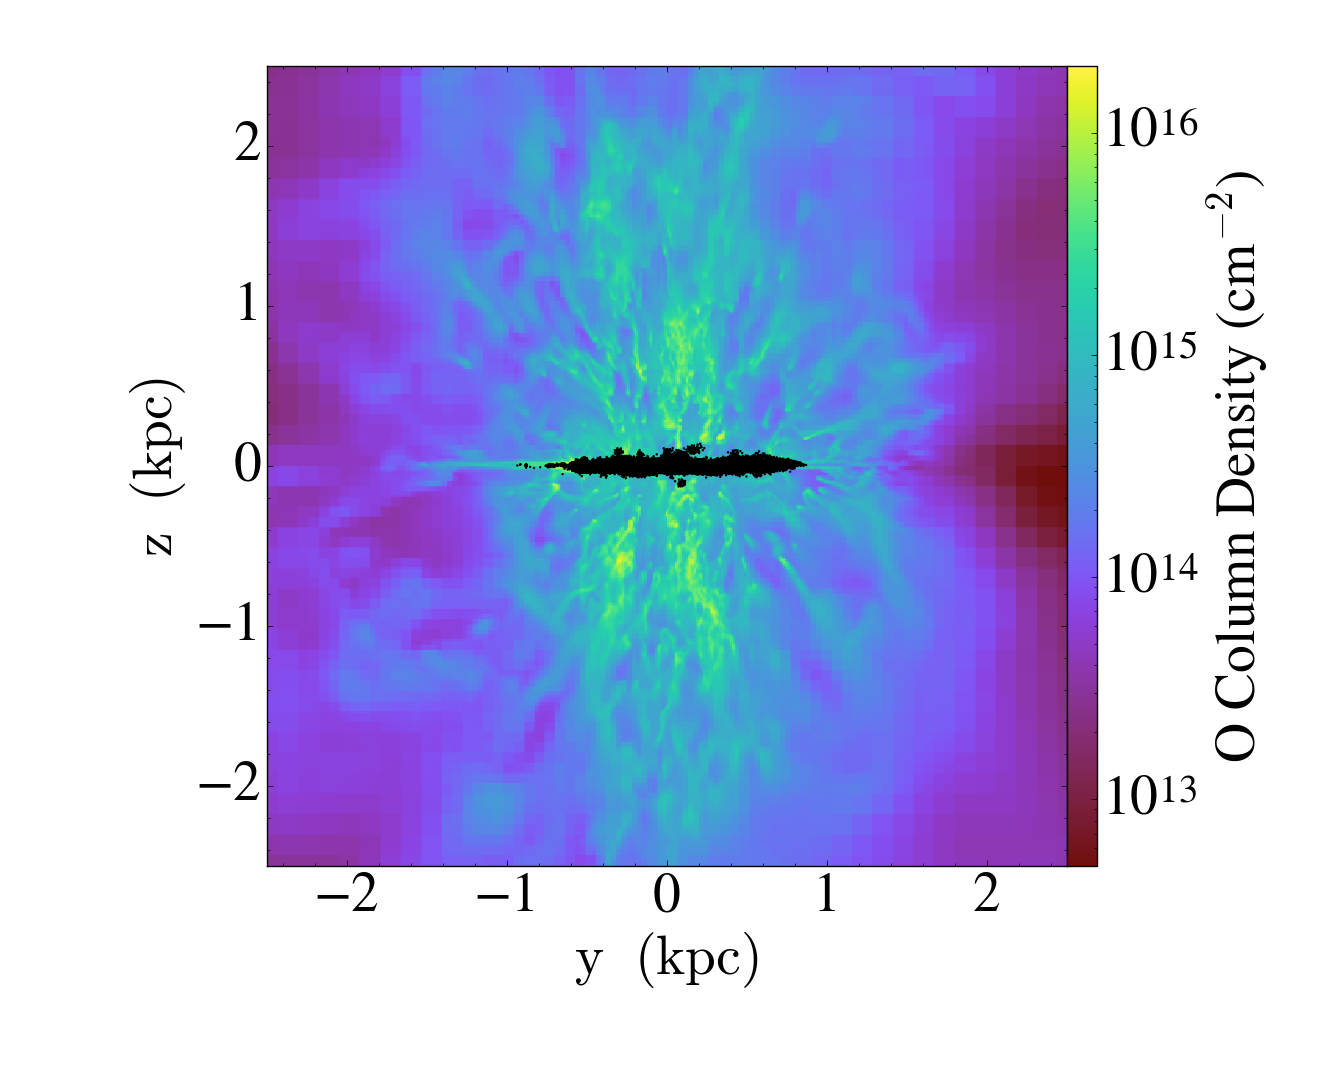
\includegraphics[width=0.4\linewidth]{O_proj_snwind}
\caption{\small Example galaxy edge-on projections of number density (weighted by density) and O column density (integrated projection) from a proof of concept test of our most massive dwarf galaxy model (M$_{\rm gas} = 10^{7}$ M$_{\odot}$) run at low resolution (8 pc) with full feedback physics (left column) and without radiation (right column). Each image shows the galaxy $\sim$ 200 Myr after first star formation, with individual stars plotted as black points. Already there is stark contrast between these two cases. The full feedback physics simulation effectively removes a substantial amount of gas from the galaxy, quickly dropping the star formation rate, and more effectively ejects produced metals from the galaxy disk. For comparison, the full physics simulation has formed $4.36 \times 10^{4}$ M$_{\odot}$ worth of stars by this point, while the simulation without radiation feedback has formed substantially more, $3.22 \times 10^{5}$ M$_{\odot}$. At its peak, the full physics simulation had 265 ionizing sources.}
\label{fig:dwarf galaxy}
\end{figure}

\section{Computational Resources}
We request a total of 2.62 million SU's, XXX TB of short term storage, and XX TB of long term storage, as explained below, for our six fiducial simulations and two additional simulations we intend to use as a resolution study. Analysis for each project will be conducted on local computing resources utilizing the open source analysis toolkit \texttt{yt} \citep{yt}, and is therefore not considered in the total SU expense.

Our primary objective is to test the role various feedback processes play in the structural, dynamical, and chemical evolution of low mass dwarf galaxies. These simulations are tied to observable properties of nearby ultrafaint dwarf galaxies through star formation history, distribution and retention of chemical ejecta, and the spatial distribution and abundances of the individual stars. This is a pivotal test of whether or not widely used, approximate feedback methods are consistent with more physical descriptions of feedback. The computational cost of these methods, and our requirement for high enough resolution to at least minimally resolve the feedback injection scales are dominant sources of computational expense. From our test runs, a maximum grid resolution of 1.5 pc offers the best balance between resolving the feedback physics and computational feasibility. These simulations will be vital for the understanding of feedback physics, and dwarf galaxy chemical and dynamical evolution, and can be used in future work to help implement physically motivated feedback methods in larger scale simulations. For example, we intend to use the results of these simulations to improve feedback prescriptions in lower resolution simulations, which will allow us to run models for Gyr time scales to better probe long term chemical evolution. We outline the parameters and cost for each of our individual runs in Table~\ref{table:SU}, and discuss them in more detail below.

\begin{table}

  \centering
  \footnotesize
  
  \begin{tabular}{| R | R | r | r | r | r | R|}
  \hline
  \multicolumn{1}{|m{1.5cm}|}{Model Number} & \multicolumn{1}{|m{1.5cm}|}{Gas Mass 10$^{6}$ M$_{\odot}$} & Radiation & Resolution (pc) & 10$^{3}$ SU/Myr & Time (Myr) & \multicolumn{1}{|m{1.0cm}|}{Total SU (10$^{6}$)} \\
  \hline
  IC* & - & - & - & - & - & 3.8$\times 10^{-3}$ \\
  1 & 2 & Y & 1.5 & 0.55 & 200 & 0.14 \\
  2 & 2 & N & 1.5 & 0.55 & 200 & 0.14  \\
  3 & 5 & Y & 1.5 & 1.4 & 200 & 0.28 \\
  4 & 5 & N & 1.5 & 1.4 & 200 & 0.28 \\
  5 & 10 & Y & 1.5 & 4.0 & 200 & 0.8 \\
  6 & 10 & N & 1.5 & 4.0 & 200 & 0.8 \\
  7 & 5 & Y & 3.0 & X & 200 & 0.09 \\
  8 & 5 & Y & 6.0 & X & 200 & 0.03 \\
  \hline
  Total & - & - & - & - & - & 2.57 \\
  \hline
  \end{tabular}
  \caption{\small List of our planned dwarf galaxy feedback simulations covering three different initial gas masses embededed in the same dark matter halo. The first row covers needed computation time to follow the collapse of each of the three dwarf galaxies (which we only need to do once per galaxy); this computation is quick and inexpensive, amounting to about 10 wall hours on 128 cores for each galaxy. We vary the feedback physics in each of our six fiducial simulations, turning on/off tracking all radiation physics from our stars (ionizing radiation, photoelectric heating from FUV radiation, and LW radiation). Our final two simulations serve as a resolution study on our feedback model.}
  \label{table:SU}

\end{table}

\begin{table}
 \centering
 \footnotesize
 \begin{tabular}{| R | R | R | R | R | R | R | R  | R }
 \hline
 \multicolumn{1}{|m{1.5cm}|}{Model Number} & \multicolumn{1}{m{1cm}|}{Number of Fields} & \multicolumn{1}{m{2.25 cm}|}{Number of Particle Fields} & \multicolumn{1}{m{2.0cm}}{Est. Number of Cells (10$^6$)} & \multicolumn{1}{m{2.0cm}|}{Memory Per Output (Gb)} & \multicolumn{1}{m{1.75 cm}|}{Short / Long Term Cadence (Myr)} & \multicolumn{1}{m{1.5cm}|}{Short Term Storage (TB)} & \multicolumn{1}{m{1.5cm}|}{Long Term Storage (TB)} \\
 \hline
  1 & 36 & 25 & 5   & 1.4  &  0.5 / 2 & 0.56 & 0.14  \\
  2 & 43 & 25 & 5   & 1.7  &  0.5 / 2 & 0.68 & 0.17  \\  
  3 & 36 & 25 & 5.4 & 1.6  &  0.5 / 2 & 0.64 & 0.16  \\
  4 & 43 & 25 & 5.4 & 1.9  &  0.5 / 2 & 0.76 & 0.19  \\
  5 & 36 & 25 & 6   & 1.7  &  0.5 / 2 & 0.68 & 0.17  \\
  6 & 43 & 25 & 6   & 2.1  &  0.5 / 2 & 0.84 & 0.21  \\
  7 & 43 & 25 & 3.7 & 1.3  &  0.5 / 2 & 0.52 & 0.13  \\
  8 & 43 & 25 & 2.4 & 0.9  &  0.5 / 2 & 0.36 & 0.09  \\
  \hline
  TOTAL & - & - & - & - & - & 5.04 & 1.26 \\
 \hline
 \end{tabular}
 \caption{\small The estimated short and long term memory storage requirements for each of our dwarf galaxy simulations, and the total storage requested for this portion of our project. Each of the above grid and particle fields are stored as a 64 bit float. The above calculations were made assuming the number of grid cells shone in each simulation, along with assuming a total number of stars each would produce assuming 2\% of the initial gas mass is converted into stars.}
 \label{table:storage}
\end{table}

We trace a total of twelve metal abundances in each simulation, restricting ourselves to those most readily constrained by observations, while adequately sampling signatures of distinct nucleosynthetic processes \citep[see][and references therein]{Tolstoy2009}: C, N, O, Mg, Si, S, Mn, Fe, Ni, Y, Ba, and Eu. We simulate three different dwarf galaxy gas masses, $2 \times 10^{6}$, $ 5 \times 10^{6}$, and $10^{7}$ M$_{\odot}$, with two simulations for each, one with and one without radiation feedback physics. We plan to conduct two additional full physics simulations with or medium mass galaxy, $5 \times 10^{6}$ M$_{\odot}$, at 3 and 6 pc resolution in order to perform a convergence test on our feedback models. 

The SU / Myr cost of each simulation is controlled by the total number of grid cells, size of each time step, and the included feedback physics (radiation or no radiation). We estimate that the high velocity stellar winds (10$^{2-3}$ km s$^{-1}$) and hot gas from supernovae and shocks (10$^{6-7}$ K) will restrict the the maximum refinement level to time steps on order of a few to several hundred years. Our test simulations at 1.5 pc resolution of each of our galaxy models show that there will be approximately $5.0 \times 10^{6}$, $5.4 \times 10^{6}$, and $6 \times 10^{6}$ cells for our least to most massive galaxies respectively. Our scaling tests show that \texttt{Enzo} operates at an average efficiency of $\sim 3.3\times 10^{3}$ and $\sim 1.2\times 10^{3}$ cell updates per second per processor for our two most massive galaxies while running at resolution with full feedback physics and $\sim$ 500 and $\sim$ 1000 radiating particles respectively. We show that these small (physical) scale simulations perform best at 128 processors in our supplemental scaling document. Given this, and typical time steps on order of 600 yr, a back of the envelope estimation gives that the two most massive simulations with full physics will cost 0.15M and 0.46M SU. A more careful estimation of the computational cost of each of these simulations (as discussed in the supplemental code performance and scaling document) shows this simple estimate is an underestimation. We anticipate the total cost in each case to be 0.28M and 0.8M SU, as shown in Table~\ref{table:SU}.

We did not perform as detailed of an estimate for the cheapest, lowest mass simulation, but expect it to be about a factor of 2 less expensive than the medium mass galaxy. We estimate our 3 parsec simulation will have $\sim 3.7 \times 10^{6}$ cells, found by adding up the number of cells in refinement levels up to 3 pc in the 1.5 pc resolution simulation, plus one eighth of the number of cells in the highest level of refinement. Likewise, the 6 pc simulation will have about $\sim 2.4 \times 10^{6}$ cells. The typical time step in the 3 pc and 6 pc resolution simulations will be a factor of two and four larger than that in the 1.5 pc simulation, as dt scales linearly with grid size. Thus we estimate that these simulations will be substantially less expensive, or 0.09M SU and 0.03M SU respectively.

Although using radiative transfer does incur substantial additional cost, radiative feedback can be very effective in shutting off star formation in these galaxies (see our low resolution test in Figure~\ref{fig:dwarf galaxy}). This means that the additional cost of following radiation is offset, since the simulation ultimately follows less star particles. While this is fortunate, it makes properly estimating the cost of the simulations with no radiative feedback challenging. Performing an accurate estimate of this cost would require running a pair of these simulations at resolution for at least 10's of Myr to observe how the complicated process of feedback regulated star formation plays out in these galaxies, which is the goal of this proposal in the first place. For this reason, we make the assumption that the non radiative feedback simulations will cost approximately the same as the full radiation feedback simulations; whatever these gain in not having to follow radiative transfer will be lost by having to track many more additional star particles. 

%Tracking CR energy density adds little additional computational cost per timestep, but will decrease the typical timestep by a factor of about 5, thus increasing the total cost by about 5. 

We plan to run each simulation for 200 Myr, saving data dumps every 0.5 Myr. We estimate that this cadence is necessary to provide access to a few restart dumps within a single job submission (depending on the included physics). Rapid analysis of this high cadence will allow us to understand the short timescale variance of dwarf galaxy chemodynamics; these will also be used to make high time resolution movies of our simulation set. Each output contains all of the information about the simulation at a single time. The memory required for each dump varies depending on the physics used, as follows. Each simulation dump will contain 12 fields associated with the hydrodynamics and 22 fields associated with the primordial chemistry and metal abundance tracers, for a base total of 34. Radiative transfer (ionizing radiation) simulations will contain an additional 7, while photoelectric heating and Lyman Werner radiation add an additional 2, for a total of 43 fields per cell in our full simulations. In addition, each particle keeps track of 25 properties, 15 of which are abundances (metallicity, H, He, and metal tracers), while the rest include position (3), velocity (3), current mass, birth mass, lifetime, and formation time; we expect on order of 10$^{4}$ to a few by $10^{5}$ star particles in our dwarf galaxies at the end of 200 Myr. Taking into account these values, our output cadence, the expected number of grid cells in each simulation, and the expected number of star particles, we present our estimated memory storage requirements in Table~\ref{table:storage}. \texttt{Enzo} operates in double precision; to ensure accuracy during restarts and to prevent loss of precision, each of our output dumps will also be in double precision.

\section{Project team qualifications}

\textbf{PI: Mordecai-Mark Mac Low}  is a tenured curator in the Department of Astrophysics at the American
Museum of Natural History in New York, as well as holding an adjunct professorship in the Department of 
Astronomy at Columbia U.  He was awarded a Humboldt Prize to visit the University of Heidelberg in 2015-2016.
He worked with and participated in the
development of the astrophysical MHD code Zeus starting in 1986, including
developing a module to include ambipolar diffusion
% (Mac Low et al. 1995; Mac Low \& Smith 1997), 
\citep{MacLow1995,MacLowSmith1997} and writing the first version of MHD
for Zeus-MP 
%(Hayes et al.\ 2006)
\citep{Hayes2006}.  He has also published work using GADGET 
%(Li, Mac Low \& Klessen 2005ab, 2006).  
\citep{Li2005,Li2005a,Li2006},
the Pencil code 
%(Oishi, Mac Low, \& Menou 2007; Johansen et al.\ 2007; Johansen, Youdin, \& Mac Low 2009; Yang, Mac Low, \& Menou 2009; Oishi \& Mac Low 2009,McNally et al. 2014), 
\citep{Oishi2007,Johansen2007,Johansen2009,Yang2009,OishiMacLow2009,McNally2014}, and
Flash 
%(Joung \& Mac Low 2006; Joung et al.\ 2009;Peters et al.\ 2010abc, 2011, 2012, Hill et al. 2012),
\citep{Joung2006,Joung2009,Peters2010,Peters2010a,Peters2010b,Peters2011,Peters2012,Hill2012,Gatto2015,Girichidis2016SImulatingOutflows,Ibanez-Mejia2016}, and Enzo \citep{Simpson2013}.
In
total, he has published over 130 refereed papers. He is co-supervisor of the dissertation work of both co-PIs, and
will supervise the work proposed here, ensuring completion and publication.

\textbf{co-PI: Andrew Emerick} is a PhD student at Columbia University advised by both PI Mac Low and collaborator Greg Bryan. Emerick is the developer of the new star formation, feedback, and stellar yield models used in the isolated dwarf galaxy simulations and drafted these sections of the proposal. This work is the central focus of his thesis research. Previously he has published research working with \texttt{ENZO}, making synthetic absorption observations of gas in simulated galaxy clusters \citep{Emerick2015}, \texttt{FLASH}, studying gas stripping and feedback in low mass dwarf galaxy satellites of the Milky Way \citep{Emerick2016}, and has authored pieces of the \texttt{Grackle} library \citep{Grackle} that are relevant to this work.

\textbf{Collaborator: Greg Bryan} is a professor at Columbia University and a Group Leader at the Simons Center for Computational Astrophysics at the Flatiron Institute. Bryan was the original author of the \texttt{Enzo} simulation code, and continues to play an active role in its development. % {\bf additional text / rewording TBD}.

\section{Management}

\subsection{Summary}

Code development, production, and analysis of simulations of star formation, feedback, and chemodynamics of isolation galaxies in \texttt{Enzo} will be led by co-PI Emerick. These simulations will be supervised by PI Mac Low and collaborator Greg Bryan. This project relies on collaboration and advice from many additional researchers, including Brian O'Shea (Michigan State), Benoit C{\^o}t{\'e} (Michigan State), Mary Putman (Columbia), Kathryn Johnston (Columbia), Britton Smith (Edinburgh), John Wise (Georgia Tech), and Simon Glover (ITA-Heidelberg).

\subsection{Local Computing Environment}

The PI's group has an analysis workstation containing  2 AMD 6344 Abu Dhabi processors with 12 cores each, 256 GB of memory, 16 TB of data space, about 40 GB of home directory space, and an Nvidia GeForce GT 610 graphics card. It is running Ubuntu, and has all standard libraries installed.  The PI and his group also have partial access to two small clusters at the Museum. These include a 128 core (32 nodes each with two dual core processors) Xeon cluster connected with Infiniband, and a 40-processor Sunfire Ultrasparc III 900 Mhz cluster. These aged machines are shared with other users at the Museum including biologists doing large phylogenetic computations, and other astrophysicists.

Through the Department of Astronomy at Columbia University, co-PI Emerick has partial access to Yeti, a 2762 core (167 nodes with dual, 1.8 Ghz, 8 core processors) HPC cluster. A subset, 64, of these nodes are connected via Infiniband. Resources on this cluster are shared between several departments at Columbia on a department-by-department basis. The ease of access coupled with fairly short to no queue wait times makes this an ideal resource for code development, testing, and some analysis work. However, resource availability and ``fair-use'' principles make using Yeti for production level simulations prohibitive. Some short term storage is available on this cluster, but is severely limited; a total of 5 TB is shared between $\sim$ 50 users.

\subsection{Other Supercomputing Support}
 
co-PI Emerick has an active 1000 SU trial allocation on the XSEDE resource Comet.
\clearpage
\appendix

\section{Introduction}

We determine the performance and scaling properties of \texttt{Enzo} in the context of the typical computational loads of our intended isolated dwarf galaxy simulations. In this situation, we are concerned with the weak scaling properties and efficiencies of \texttt{Enzo}. This analysis makes use of case studies of our dwarf galaxy model run at our intended resolution of 1.5 pc, and is based on past experience with 1.0 pc, 2.0 pc, and 8.0 pc resolution tests. Unless otherwise noted, these tests ran on 128 processors on the TACC Stampede cluster, our proposed allocation resource.

\subsection{Computational Methodology and Algorithms}

\texttt{Enzo} is a parallel, cosmological, AMR hydrodynamics + N-body code that has been well tested and used in a variety of applications, as discussed in more detail in the main document. Below, we outline the code methodology for each piece of \texttt{Enzo} relevant to this present work; see \cite{Enzo2014} for a more detailed description of all methods. 

\subsubsection{Hydrodynamics and Gravity}

\texttt{Enzo} is equipped with multiple, distinct hydrodynamics solvers. For this work we employ a direct-Eulerian piecewise parabolic method \citep{ColellaWoodward1984, Bryan1995}. This is an explicit, higher-order accurate version of Godunov's method for ideal gas hydrodynamics. This base method is extended to multiple dimensions using directional splitting, resulting in a final algorithm that is second-order accurate in space and time; we explicitly conserve mass, linear momentum, and energy. We default to using the two-shock approximate Riemann solver, with progressive fallback to more diffusive approximate Riemann solvers when higher order methods produce negative densities or energies. The hydrodynamics time step is set by the Courant-Friedrichs-Levy (CFL) condition for stability, scaling linearly with cell size ($\Delta x$) and inversely proportional to the sum of the bulk velocity and sound speed in each cell in a given direction. 

%\texttt{Enzo} is equipped with multiple, distinct hydrodynamics solvers. For this work we employ a direct-Eulerian piecewise parabolic method \citep{ColellaWoodward1984, Bryan1995}. This is an explicit, higher-order accurate version of Godunov's method for ideal gas hydrodynamics that uses spatially third-order accurate piecewise parabolic monotonic interpolation. Shock capturing is handled with a nonlinear Riemann solver. This base method is extended to multiple dimensions using directional splitting, resulting in a final algorithm that is second-order accurate in space and time; we explicitly conserve mass, linear momentum, and energy \citep{Hawley1984, NormanWinkler1986}. We use a dual energy formalism to track the total energy and thermal energy separately, preventing substantial numerical errors that arise when the thermal energy is very small compared to the total energy (i.e. when the kinetic energy is large). We default to using the two-shock approximate Riemann solver \citep{Toro1997}, with progressive fallback to more diffusive approximate Riemann solvers when higher order methods produce negative densities or energies \citep{LemasterStone2009}. In this situation, we fall back to either the Harten-Lax-van Leer (HLL) \citep{Toro1997} method with contact discontinuities -- a three-wave, four-state solver -- or the basic HLL -- a two-state, three-wave solver. The hydrodynamics time step is set by the Courant-Friedrichs-Levy (CFL) condition for stability, scaling linearly with cell size ($\Delta x$) and inversely proportional to the sum of the bulk velocity and sound speed in each cell in a given direction. The multidimensional CFL limited time step is the harmonic average of the limiting CFL time step in each dimension. 

%Gas self-gravity and the gravitational forces of the massive star particles are computed together to compute the gravitational acceleration on each cell and particle. On the root grid, we use a cloud-in-cell (CIC) method \citep{HockneyEastwood1988} to map particles to a time-centered density field, including the effects of particles across sub-grids and neighboring domains; a similar time-centered density field is computed for the baryons in each grid cell. The gravitational potential is solved for using a fast Fourier transform (FFT) in isolated boundary conditions \citep{James1977}; accelerations are computed with a two-point centered difference scheme using the transformed real-space potential. For accuracy on sub-grids, we employ the seven-point, second-order finite difference approximation to Poisson's equation, solving the given Dirichlet boundary conditions with multigrid relaxation. Unwanted oscillations and errors across grids are reduced using expanded buffer zones around each grid, coupled with an iterative relaxation process between sibling grids. Particle accelerations are computed from the grid potential using linear CIC mapping. \texttt{Enzo} employs the particle-mesh N-body method from \cite{HockneyEastwood1988} to evolve the colissionless star particles with an effective force resolution of approximately 2$\Delta x$.

\texttt{Enzo} constructs the gravitational potential from both the gas and star particles to compute the resulting accelerations for each cell and particle. Particles are mapped to a time-centered density field using a cloud-in-cell (CIC) method \citep{HockneyEastwood1988}; this is summed together with a time-centered baryon density. The potential is solved on the root grid using a fast Fourier transform with isolated boundary conditions \citep{James1977}. For accuracy on sub-grids, we solve an approximate Poisson's equation with a second-order finite difference method and multigrid relaxation. Baryon accelerations are computed using a two-point centered difference scheme; accelerations are mapped to particles using linear CIC interpolation. \texttt{Enzo} employs a particle-mesh N-body to evolve the colissionless star particles with an effective force resolution of $\sim 2 \Delta x$.

\subsubsection{Grid Hierarchy and Parallelization Strategy}

%\texttt{Enzo} AMR simulations begin with a defined rectilinear root grid encompassing the computational domain. Additional levels of refinement take the form of child sub-grids nested within the root grid, generating a nested tree comprised of grid parents, children, and siblings; for our purposes, additional sub-grids increase resolution by a factor of two. Each grid is comprised of active zones and ghost zones that store boundary information from sibling grids. Each level in this tree is evolved on independent time steps, reducing unneeded computation on lower levels of refinement.

\texttt{Enzo} AMR simulations begin with a rectilinear root grid encompassing the computational domain. Additional levels of refinement take the form of child sub-grids, nested within the root grid; the grid hierarchy then consists of parent, child, and sibling grids. Grids contain both active and boundary (ghost) zones used for sharing sibling grid information. Each level in the grid hierarchy is evolved on independent time steps, reducing unneeded computation. 
%Using grid objects as fundamental units that exist entirely on a single processor, \texttt{Enzo} has been parallelized with the message passing interface (MPI). Grids are therefore distributed among processors in such a way to attempt to balance the computational load across processors. This is simple for the root grid, which is evenly divided in tiles to all processors, but is more complicated for higher refinement levels, which usually are not uniformly distributed in the simulation volume. Higher levels of refinement are initially placed on the processors that host their parent grids, but are subsequently distributed among other processors to reduce computational load. Load is estimated as the number of active zones on each grid. We use a simple load-balancing option to progressively move grids from processors with high computational loads to processors with the lowest computational loads until the load ratio of the most-to-least loaded processors is less than 1.05. To improve performance further, \texttt{Enzo} dynamically adjusts the size of each sub-grid on a given level depending on the number of zones on the given level and the load balance across processors on that level. This reduces communication time across processors on each level while also improving the effectiveness of load-balancing. 
Grid objects, the fundamental units of the hierarchy and parallelization strategy, exist entirely on a single processor. Grids are distributed to balance computational load across processors. The root grid is evenly distributed across all processors, but grids at higher levels of refinement are shifted across processors such that the load ratio between the highest and lowest loaded processor is less than 1.05. Dynamically sized sub-grids on a given level provide \texttt{Enzo} with an additional degree of freedom in the load-balancing strategy.

All processors contain a copy of the entire grid hierarchy meta data, allowing for easy non-blocking communication across processors; the additional memory overhead of storing this data on each processor is negligible. In addition, all star particle information is stored on each processor (again, with negligible memory overhead), removing the need for communication when injecting feedback from stars close to grid boundaries.

\subsubsection{Radiative Transfer Methods}

%\cite{WiseAbel2011} implemented radiative transfer capabilities in \texttt{Enzo}, performing rigorous tests of its capabilities, and has been used in a variety of applications \citep[e.g.][]{Wise2012a,WiseAbel2012,Wise2014, Smith2015, OShea2015, Koh2016, Regan2016a, Regan2016b}. The equations of radiative transfer are solved directly on the computational domain following directly traced rays from individual point sources. This is an inherently computationally expensive process. To improve efficiency \texttt{Enzo} employs an adaptive ray tracing method \citep{AbelWandelt2002} where rays are mapped from a point source to HEALPix pixels surrounding the source. The resulting rays are advanced through the grid, progressively refining rays by splitting them into child rays once the ratio of the cell face area to ray solid angle drops sufficiently. In a given time step, rays propagate a distance $c\times dt$, or until they either leave the computational domain or their flux drops by 99.99\% or more in a single cell. If the rays still exist at the end of the ray tracing step, their evolution is halted and stored for the next time step. The resulting ionization and heating rates due to the radiation field are computed assuming the photo-ionization and absorption rate are equal, ensuring photon conservation \citep{Abel1999, Mellema2006}. These are passed to the \texttt{Grackle} chemistry solver to update the correct ionization, chemical, and energy states in each cell.

\cite{WiseAbel2011} implemented radiative transfer (RT) capabilities in \texttt{Enzo}, performing rigorous tests of its capabilities, and has been used in a variety of applications \citep[e.g.][]{WiseAbel2012,Wise2012a,Wise2014, Smith2015, OShea2015, Koh2016, Regan2016a, Regan2016b}. The equations of RT are solved directly following rays traced from individual point sources. This inherently expensive process is computed efficiently with an adaptive ray tracing method \citep{AbelWandelt2002}. Rays are advanced outward from a mapping to HEALPix pixels around the source, progressively split and refined to child rays far from the source. Rays travel $c\times dt$ in a time step, and are removed if their flux drops by 99.99\% or more in a cell. Ensuring photon conservation \citep{Abel1999,Mellema2006}, ionization and heating rates are self-consistently processed in the \texttt{Grackle} chemsitry solver to update the correct ionization, chemical, and energy states in each cell.

%\subsubsection{Cosmic Ray Transport}

%Cosmic ray (CR) feedback and transport was implemented in \texttt{Enzo} in \cite{SalemBryan2014}, and has since been used in multiple studies of its effects on galaxy evolution \citep{SalemBryanHummels, SalemBryanCorlies, Chen2016}. CR's are modeled with a two-fluid method \citep{Drury1985, DruryFalle1986,Jun1994}; the CR fluid is evolved as a $\gamma = 4/3$ ideal gas as usual, yet is coupled directly to the thermal gas hydrodynamics via an additional pressure term. CR energy density is allowed to diffuse at a rate controlled by an input diffusion coefficient, $\kappa_{\rm CR}$. This equation is solved using an explicit finite-difference scheme, creating a $\Delta x^2$ dependence on the limiting time step size for CR evolution. At high resolution, this restriction can be a factor of a few to several times smaller than the limiting hydrodynamics time step. To mitigate this slow down, CR evolution is sub-cycled on each grid for either a full hydrodynamics time step, or up until communication across grids would be required (controlled by the number of boundary ghost zones used on each grid). This ultimately limits the effectiveness of sub-cycling, but still shows an improvement by a factor of 2-5 in run time as compared to non sub-cycled simulations.

%Cosmic ray (CR) feedback and transport was implemented in \texttt{Enzo} in \cite{SalemBryan2014}, and has since been used in multiple studies of its effects on galaxy evolution \citep{SalemBryanHummels, SalemBryanCorlies, Chen2016}. CR's are modeled with a two-fluid method \citep{Drury1985, DruryFalle1986,Jun1994}. The CR diffusion is solved using an explicit finite-difference scheme, creating a $\Delta x^2$ dependence on the limiting time step size for CR evolution. This can be expensive at high resolution. To improve speed, CR's are sub-cycled within each grid up until a communication step is required, providing a factor of 2-5 improvement over non sub-cycled runs.


\subsection{Performance and Scaling of AMR Simulations}

%Profiling the exact scaling and performance properties of an AMR simulation is challenging, as the total number of computational grids can vary significantly over the course of the simulation run. In the case of our dwarf galaxy simulations, the number of grids will initially be relatively insignificant, but will grow substantially once the gas collapses to high densities and forms stars. Based on our test simulations, we expect the number of grid cells to be roughly consistent from this point onward, fluctuating around some mean value. Given a roughly constant cell count, code performance (number of cell updates per second per processor) will be roughly consistent, with computational expense (SU per simulation Myr) set by the size of each time step. As discussed above, time steps are set independently on each refinement level; in general the hydrodynamics time step will be the limiting constraint due to the presence of hot, fast moving gas from stellar winds and supernovae. The additional expense of following radiative transfer correlates with the number of ionizing sources, yet depends on how these sources are clustered spatially (clustering limits how evenly these sources can be distributed among processors). We refer to the main document for further details on how this affects the anticipated cost of our simulations.

Profiling the exact scaling and performance properties of an AMR simulation is challenging, as the total number of computational grids can vary significantly over a run. In our case, the number of cells will initially be small, growing significantly once our galaxy collapses and reached star forming densities. Eventually, the total cell count will equilibrate with fluctuations. Code performance (cell updates per second per processor), at this point, will be roughly consistent, while computational expense (SU per Myr) will be controlled by $\Delta t$ on each level. The hydrodynamics time step is often the limiting factor, due to hot, rapidly moving gas from feedback sources. RT adds additional expense, correlating with the number and clustering of ionizing sources.

%\subsection{Code Performance and Grid Hierarchy}



%We begin by illustrating how our computational domain is divided between individual levels in an AMR run of our dwarf galaxy. Figure~\ref{fig:levels} shows the results of two test simulations of our dwarf galaxy in a slightly larger box than our planned simulation ($16.384^3$ kpc with a $128^3$ root grid instead of $12.288^3$ kpc) at a maximum refinement level of 6 and 7, corresponding to a physical resolution of 2.0 and 1.0 pc respectively. As demonstrated, the amount of wall time spent on a single cycle is dominated by computation on the highest level of refinement (top left panel). This is because the number of cells on a given level generally increases towards higher levels of refinement (top right panel), with the most cells on a given level at the highest refinement level, and because the time step is allowed to vary on each level, scaling linearly with the cell size. In reality, the typical timestep scales much more steeply with refinement level as the feedback physics (with hot gas and high velocities) is injected at the maximum resolution, and we expect most of the cells in the root grid to be sufficiently far from the galaxy to be devoid of any hot, fast moving gas. 

\begin{figure}
\centering
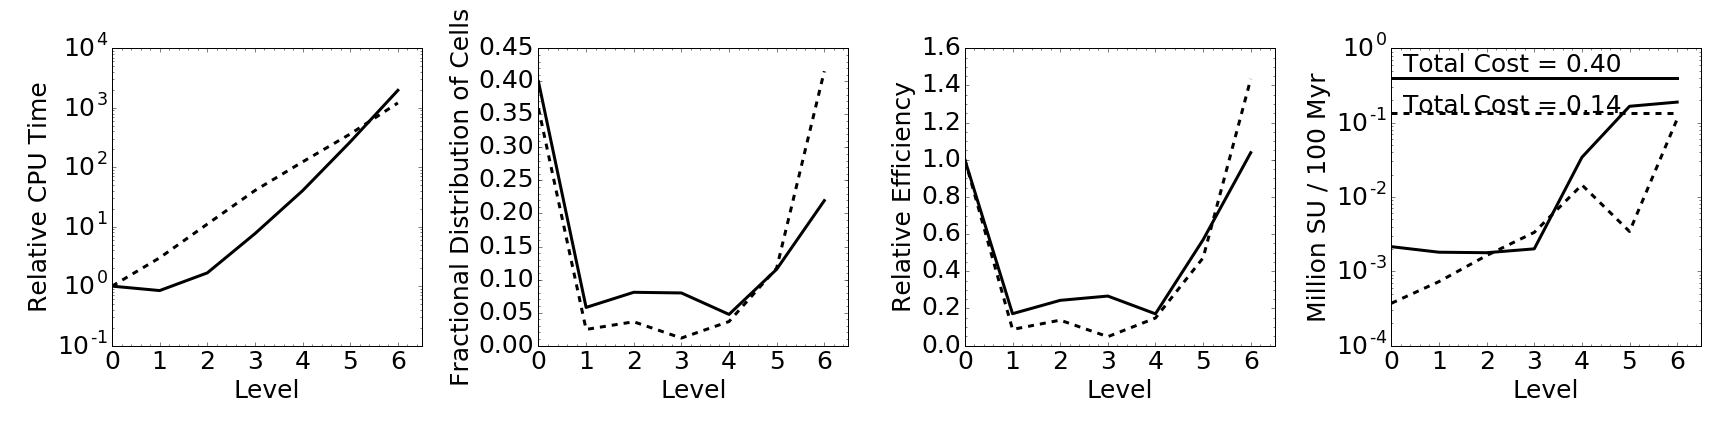
\includegraphics[width=.9\linewidth]{enzo_levels}
\caption{\small Demonstration of grid hierarchy and performance per level on a 1.5 pc simulation of our medium mass galaxy model, M$_{\rm gas} = 5 \times 10^{6}$ M$_{\odot}$, and most massive galaxy model, M$_{\rm gas} = 10^{7}$ M$_{\odot}$, in dashed and solid lines respectively. In each case, the performance profiling was taken on cycles running with full feedback physics for over 10$^{4}$ stars, and about 500 and 1000 radiating particles respectively. For each level, the first panel gives wall time spent, the second the fractional number of cells, the third the efficiency (normalized to the root grid), and the fourth the estimated total cost per 100 Myr of simulation time.}
\label{fig:levels}
\end{figure}

Figure~\ref{fig:levels} demonstrates the level-by-level break down of a single cycle in two test simulations of our M$_{\rm gas} = 5 \times 10^{6}$ M$_{\odot}$ and M$_{\rm gas} = 10^{7}$ M$_{\odot}$ galaxies run with full feedback physics, with over 10$^4$ star particles in each case. During this cycle, about 500 and 1000 of these particles were radiating in each case. The left two panels show that wall time is dominated by computation on the highest level of refinement, in large part because it dominates the cell count across levels, but also because the time step decreases linearly with resolution (not shown). Efficiency varies per level (third panel), but is high for large grid counts, demonstrating effective load-balancing. \texttt{Enzo} reaches typical efficiencies of $\sim 2 \times 10^{4}$ cell updates/s/processor when no feedback physics is used, dropping to 1-3 $\times 10^3$ when star formation and feedback occurs (as shown here). Given these efficiencies and typical values for the time step size on each level (not shown, but is approximately 600 years on the highest level of refinement), the bottom right panel shows the estimated SU cost per 100 Myr of simulation time on 128 processors on the TACC Stampede cluster. Since we plan to run for 200 Myr, the total cost for each of these simulations will be a factor of two higher than the values shown.

%The lower left panel of Figure\ref{fig:levels} provides the relative efficiency of each level, as normalized to the efficiency of level 0. We define efficiency as the number of cell updates per second per processor, with typical values of 10$^4$ as averaged over all levels. The efficiency is determined primarily by the ability of \texttt{Enzo} to properly load balance across all processors, which becomes inefficient if there are too few cells on a given level. For example, levels 1 and 2 have low cell counts and low efficiencies; however, low efficiencies for this reason are generally irrelevant, as very little time is actually spent updating these cells. The efficiency at he highest levels of refinement is generally around $2\times 10^4$ cells/s/proc. Assuming all levels can operate completely independently (which is physically impossible), we present the theoretical lower limit cost of 1 Gyr of simulation time per level on 128 cores in the lower right panel; the horizontal line gives the sum over all levels. To compute this, we adopt typical time steps for each level as obtained from our test simulations using only supernovae feedback and stellar winds. This means a typical time step of roughly 300 years at level 7, and 600 years at level 6. In practice, the levels cannot operate independently; a more realistic estimate is a factor of 2-3 larger than this theoretical minimum.

%\begin{figure}
%\centering
%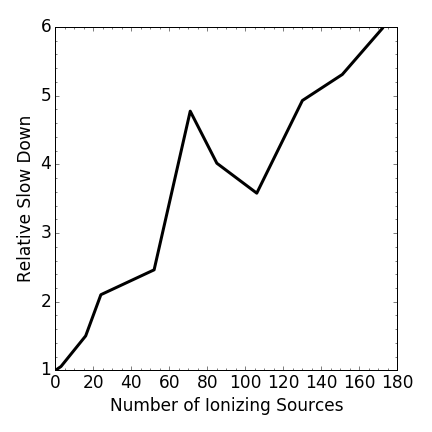
\includegraphics[width=0.45\linewidth]{enzo_radiation}
%\caption{Estimate of relative slow down of a test simulation as a function of the number of ionizing sources. The test simulation is of our dwarf galaxy at 8.0 pc resolution, or a maximum refinement level of 4, run on 32 processors on the TACC Stampede cluster. This test simulation included supernovae, stellar winds, photoelectric heating, and radiative transfer. We estimate that there will be at most a few hundred sources at any one moment in our simulation, implying a maximal slow down of about a factor of 10.}
%\label{fig:radiation}
%\end{figure}

%The left panel in Figure ~\ref{fig:radiation_and_scaling} illustrates the estimated slow down due to RT as a function of the number of ionizing particles. This test was performed in \texttt{Enzo} on our dwarf galaxy model at 8.0 pc resolution (4 levels of refinement) on 64 processors. Slow down is computed relative to the case with no radiative particles, with efficiency defined here as number of cell updates/s/particle. Additional computational time is due mostly from evolving (tracing) the individual rays and the associated additional communication across processors. Since the RT methods in Flash were based on those used in this test case, we expect similar scaling properties in this code.

%We demonstrate the effects of including radiative transfer as a function of the number of ionizing particles in Figure~\ref{fig:radiation} for a test simulation run with a maximum refinement level of 4 (8.0 pc resolution) on 64 processors. Shown is the slow down of a given cycle as a function of the number of ionizing sources. We compute this as the number of cell updates per second per particle, normalized to the zero particle case. This implicitly assumes that any decrease in performance is due solely to the number of sources, and no other factors. To be clear, the additional computational time incurred by including radiation is split in into three parts, 1) evolving the photon packages through the grid cells, 2) ray tracing from each source to deposit the photon packages, and 3) communication time communicating photon packages between processors. For this reason, the additional cost also depends upon the nature of the sources themselves, their clustering, and the details of the medium the photons propagate through.

\subsection{Scaling Tests}

\begin{figure}
\centering
%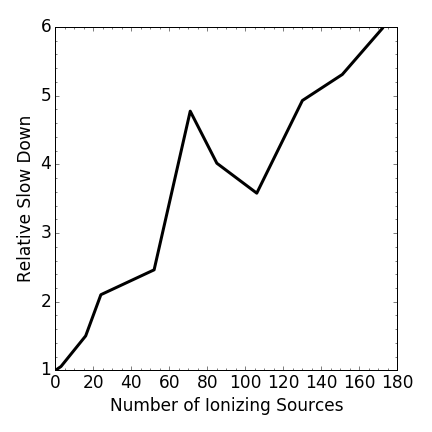
\includegraphics[width=0.32\linewidth]{enzo_radiation}
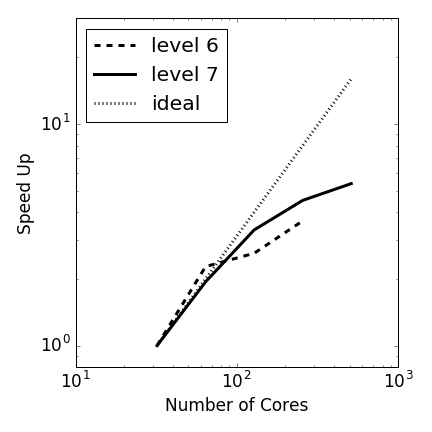
\includegraphics[width=0.32\linewidth]{enzo_scaling}

\caption{\small \textbf{Strong scaling} properties in our most massive galaxy in \texttt{Enzo} run with 6 and 7 levels of refinement at 2.0 pc and 1.0 pc resolution. Note these scaling tests are from a different simulation set than those presented in Figure~\ref{fig:levels}. We expect scaling properties for our 1.5 pc simulations to be in between those shown here. Given this, we anticipate to run on 128 cores for all of our simulations.}
\label{fig:radiation_and_scaling}
\end{figure}

We demonstrate \textbf{weak scaling} ({\it is this weak or strong scaling? }) in Figure~\ref{fig:radiation_and_scaling} for two test simulations, each run with a maximum of 6 and 7 levels of refinement, as compared to ideal scaling. Our simulations scale well up to about 128 processors, falling away from ideal at higher processor counts. However, this is in part because scaling in \texttt{Enzo} works best when the number of root grids on a side is greater than or equal to the number of cores. In this case, we don't expect perfect scaling much above 128 cores for our 128$^3$ simulations. For this reason, we anticipate to run all of our dwarf galaxy models on 128 cores. We note that \texttt{Enzo} has been shown to scale well to at least 10$^3$ processors in a variety of contexts, but the small physical size of our simulation and complexity of feedback physics do not lend themselves to scaling to very large processor counts.

\clearpage
\bibliographystyle{apj}
\bibliography{msAllbib}


\end{document}
